\section{Critical rate and an exact decomposition}
\label{sec:decomposition}

\subsection{Setting}
We use the setting of Ref.~\cite{namba2026arrow}. Phase space is $\mathbb R^d$, $d = 2n$, with dimensionless canonical coordinates $z = (q,p)$, and $\dot z = f(z)$ is a Hamiltonian flow, so that $\nabla\cdot f = \tr Df = 0$. Let $X \sim \rho_t$ be the fine-grained state and $Y = X + \sigma Z$ with $Z \sim \mathcal N(0,I)$ independent of $X$. The coarse-grained density $\rho_C$ is the density of $Y$ and $S_C = h(Y)$ its differential entropy. We write $s = \nabla\ln\rho_C$ for the score, $F = \E[s(Y)s(Y)^{\mathsf T}]$ for the Fisher information matrix, and
\begin{equation}
H(y) = -\nabla^2\ln\rho_C(y)
\label{eq:H}
\end{equation}
for the \emph{local} Fisher matrix. Throughout we assume the regularity needed for the integrations by parts below and finite moments of the quantities involved ($\E\|Df(X)\|$, $\E[|f(X)|\,|X|]$ and, in Sec.~\ref{sec:bound}, fourth posterior moments); then $\E[H(Y)] = F$. The symmetric strain rate is $\kappa = \sup_z\lambda_{\max}[\Sym Df(z)]$.

For an isotropic window that coarsens at rate $r = \dot\sigma/\sigma$, Lemma~1 of Ref.~\cite{namba2026arrow} gives $dS_C/dt = r\,\sigma^2\tr F + \Sigma$ with $\Sigma = -\E[s(Y)\cdot f(X)]$. We define the \emph{critical rate} of the state,
\begin{equation}
R = -\frac{\Sigma}{\sigma^2\tr F}, \qquad \frac{dS_C}{dt} = \sigma^2\tr F\,(r - R).
\label{eq:R}
\end{equation}
The coarse-grained entropy of the state does not decrease if and only if $r \geq R$. Conjecture~1 of Ref.~\cite{namba2026arrow} states that $R \leq \kappa$ for every state, every $\sigma > 0$ and every Hamiltonian flow with $\kappa < \infty$. For linear flows $\dot z = Bz$ one has $R = \tr(F\Sym B)/\tr F \leq \kappa$, and the supremum over states equals $\kappa$~\cite{namba2026arrow}.

Two facts about Gaussian smoothing are used throughout. First, $\Sigma = \E[\tr\Cov(f(X),X\,|\,Y)]/\sigma^2$ (Lemma~2 of Ref.~\cite{namba2026arrow}). Second, differentiating Tweedie's formula for the posterior mean~\cite{efron2011}, $\E[X\,|\,y] = y + \sigma^2 s(y)$, once more with respect to $y$ gives the second-order formula
\begin{equation}
\Cov(X\,|\,Y = y) = \sigma^2 I - \sigma^4 H(y).
\label{eq:tweedie2}
\end{equation} Because the left-hand side is positive semidefinite,
\begin{equation}
H(y) \preceq \sigma^{-2} I \qquad \text{for every } y .
\label{eq:Hbound}
\end{equation}
The coarse-grained density can nowhere be sharper than the window. Equation~\eqref{eq:Hbound} is the Euclidean form of the matrix Harnack estimate for the heat equation~\cite{hamilton1993}, with heat-kernel time $\sigma^2/2$. It bounds $H$ from above only: between separated components $H$ can be strongly negative.

\subsection{Decomposition}
Let $G(y) = \Sym\E[Df(X)\,|\,Y = y]$ be the locally averaged strain seen at $y$, and $\bar G = \E[G(Y)] = \Sym\E_{\rho_t}[Df]$ its average over the state. Define the posterior Stein defect
\begin{equation}
\Delta(y) = \Cov(f(X),X\,|\,y) - \E[Df(X)\,|\,y]\,\Cov(X\,|\,y),
\label{eq:defect}
\end{equation}
which vanishes when the posterior law of $X$ given $Y = y$ is Gaussian, by Stein's lemma~\cite{stein1981}.

\begin{proposition}[Decomposition of the critical rate]
\label{prop:decomposition}
For every state,
\begin{equation}
R = \underbrace{\frac{\tr(F\bar G)}{\tr F}}_{L}
+ \underbrace{\frac{\E\tr\!\left[(H(Y) - F)\,G(Y)\right]}{\tr F}}_{C}
+ \underbrace{\left(-\frac{\E\tr\Delta(Y)}{\sigma^4\tr F}\right)}_{D} .
\label{eq:decomposition}
\end{equation}
The law term satisfies $L \leq \lambda_{\max}(\bar G) \leq \kappa$.
\end{proposition}

\begin{proof}
Insert Eq.~\eqref{eq:defect} and Eq.~\eqref{eq:tweedie2} into $\Sigma = \E[\tr\Cov(f(X),X\,|\,Y)]/\sigma^2$:
$\Sigma = \E\tr\E[Df\,|\,Y] - \sigma^2\,\E\tr(H\,\E[Df\,|\,Y]) + \E\tr\Delta/\sigma^2$.
The first term is $\E[\nabla\cdot f(X)] = 0$. Since $H$ is symmetric, $\tr(H\,\E[Df\,|\,Y]) = \tr(H\,G)$. Hence $R = \E\tr(HG)/\tr F + D$, and writing $H = F + (H - F)$ with $\E\tr(FG(Y)) = \tr(F\bar G)$ gives Eq.~\eqref{eq:decomposition}. Because $F \succeq 0$, $\tr(F\bar G) \leq \lambda_{\max}(\bar G)\tr F$, and $\lambda_{\max}(\bar G) \leq \E_{\rho_t}\lambda_{\max}(\Sym Df) \leq \kappa$ by convexity of $\lambda_{\max}$.
\end{proof}

The covariance term $C$ is positive when the coarse-grained density is sharper than average ($H \succ F$) where the local strain is strong. In words: the observer's focus sits where the flow stretches. The Stein defect $D$ measures how far the posterior laws are from Gaussian. For a single Gaussian state both vanish (Sec.~\ref{sec:gaussian}). Rewriting Eq.~\eqref{eq:decomposition} with $A(y) = \kappa I - G(y) \succeq 0$ gives a form that shows where the conjecture can fail.

\begin{corollary}[Where the conjecture can fail]
\label{cor:where}
For every state,
\begin{equation}
\kappa - R = \frac{\E\tr\!\left[H(Y)A(Y)\right]}{\tr F} - D,
\qquad A(y) = \kappa I - G(y) \succeq 0 .
\label{eq:where}
\end{equation}
If $H(y) \succeq 0$ for all $y$, then $R \leq \kappa + D$. A state with $R > \kappa$ therefore needs either a positive Stein defect or a region where $H$ has a negative eigenvalue whose direction meets large values of $A$.
\end{corollary}

\begin{proof}
Use $\E\tr H = \tr F$ in Eq.~\eqref{eq:decomposition}. If $H \succeq 0$, then $\tr(HA) \geq 0$ because $A \succeq 0$.
\end{proof}

Regions where $H$ has a negative eigenvalue are the ``valleys'' of $\ln\rho_C$, for example between overlapping components of a mixture. For one-degree-of-freedom flows with $f = (p, g(q))$, $\Sym Df = a(q)\,\mathrm{diag}(1,-1)$ in the rotated coordinates $v = (q+p)/\sqrt2$, $w = (q-p)/\sqrt2$, with
\begin{equation}
a(q) = \tfrac12\left(1 + g'(q)\right),
\label{eq:stretch}
\end{equation}
so that $G(y) = \bar a(y)\,\mathrm{diag}(1,-1)$ with $\bar a(y) = \E[a(X_q)\,|\,y]$. We call $v$ the stretching and $w$ the contracting direction. Equation~\eqref{eq:where} then reads
\begin{equation}
\kappa - R = \frac{\E\left[(\kappa - \bar a)H_{vv}\right] + \E\left[(\kappa + \bar a)H_{ww}\right]}{\tr F} - D .
\label{eq:where1d}
\end{equation}
For the pendulum, $g(q) = -\sin q$, $a(q) = (1-\cos q)/2 \in [0,1]$ and $\kappa = 1$, attained at the hyperbolic point $q = \pi$. Figure~\ref{fig:mechanism} shows $\bar a$, the local anisotropy of $H$, the valleys and the density of the covariance term for three pendulum states.

\begin{figure*}[t]
\centering
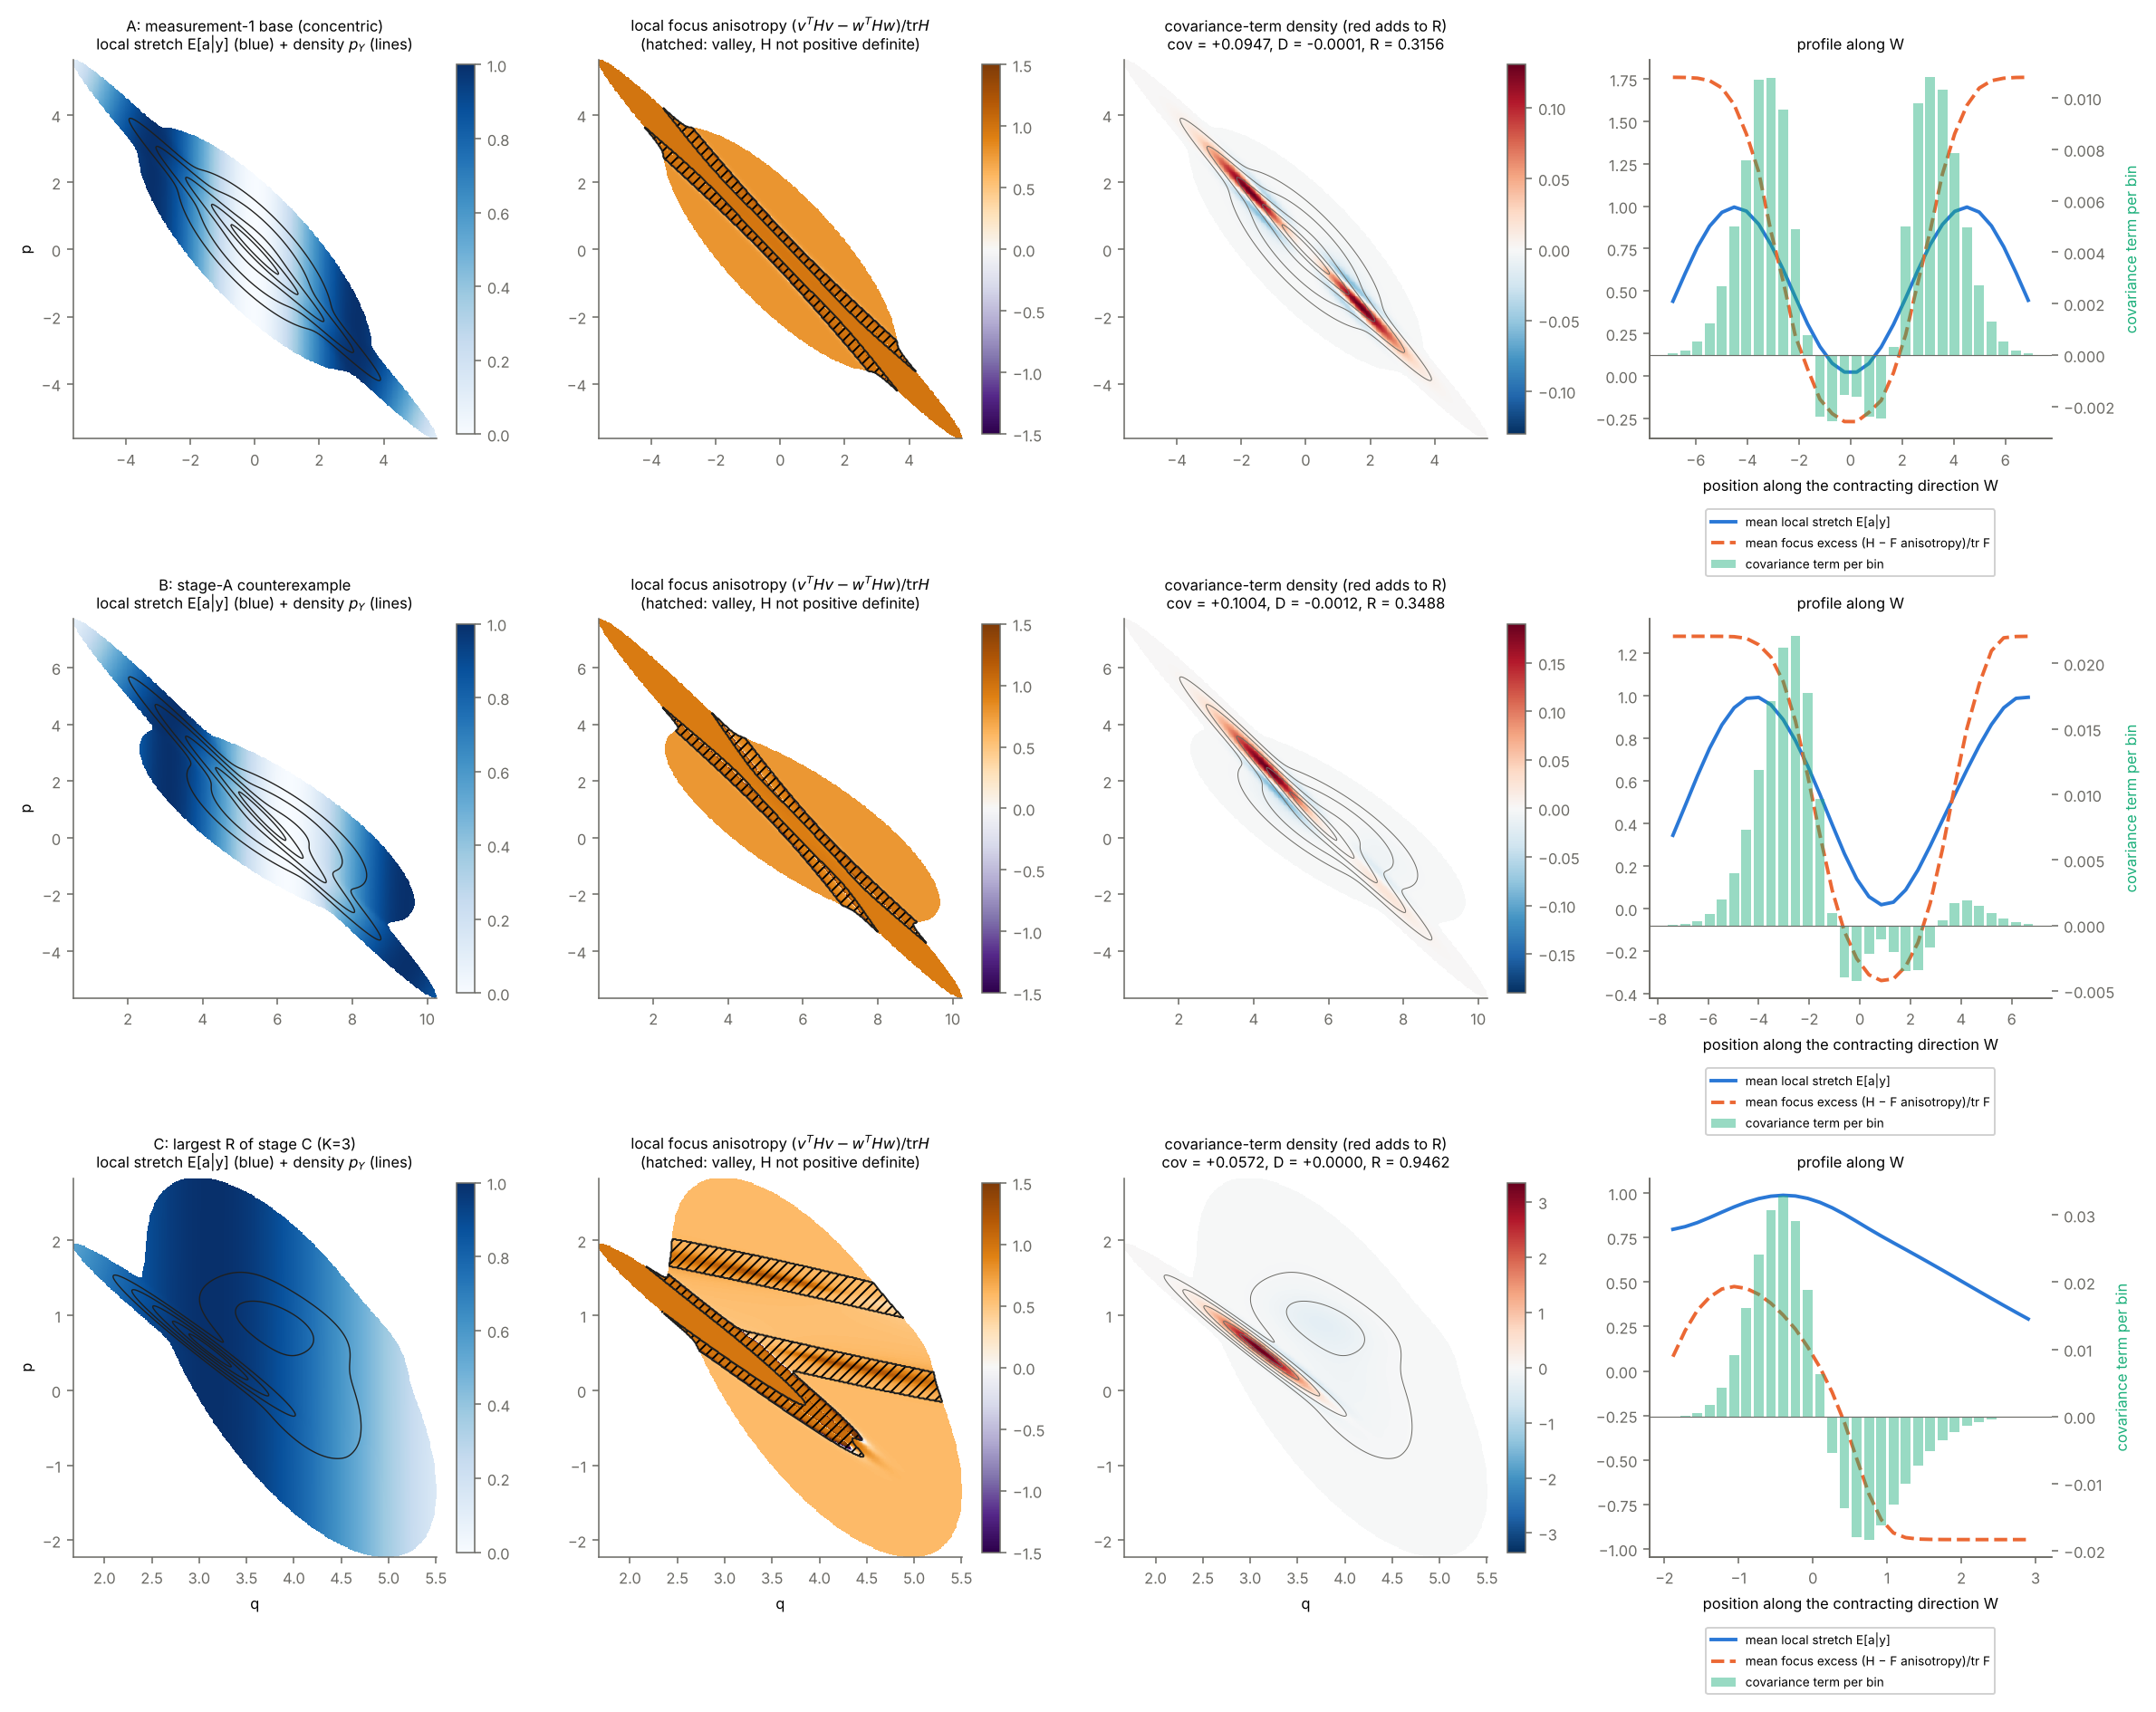
\includegraphics[width=0.95\textwidth]{figures/fig1_mechanism.png}
\caption{Mechanism of the covariance term for three pendulum states (rows). Left: local strain $\bar a(y)$ and coarse-grained density (contours). Second: local anisotropy of the focus $(v^{\mathsf T}Hv - w^{\mathsf T}Hw)/\tr H$; hatched regions are valleys, where $H$ has a negative eigenvalue. Third: density of the covariance term $C$ (red adds to $R$). Right: profile along the contracting direction. The covariance term is positive where the focus is sharp and the strain is strong.}
\label{fig:mechanism}
\end{figure*}
